\section{Approach overview}\label{approach}\noindent
Consider a computational model $\mathcal{M}$ (e.g., finite element model) with $K$ independent realisations, where $K$ is called training size. The training input $(x^{(i)})_{i=1}^K \subset \mathcal{D}_{\boldsymbol{x}}$ map to the output $\text{y} \in \mathbb{R}^N$ representing quantities of interest, such as nodal displacements or stresses:
\begin{equation}
 \label{eq:UQ_model}
 \mathcal{M}:x \in \mathcal{D}_{\boldsymbol{x}} \subseteq \mathbb{R}^M \mapsto
 \mathsf{y} = \mathcal{M}(x) \in \mathcal{D}_{\boldsymbol{\mathsf{y}}} \subseteq \mathbb{R}^N ,
\end{equation}
The inputs $\mathcal{D}_{\boldsymbol{x}}$ is low dimensional and the outputs $\mathcal{D}_{\boldsymbol{\mathsf{y}}}$ exhibit high dimensionality with spatio-temporal correlations.

\subsection{Modelling spatial correlations via compression}\noindent
Spatial pattern is a common feature in geotechnical responses, such as wall deflections in excavations, tunnel surface settlements, and pore pressure distributions in porous media. These responses exhibit strong spatial correlations dictated by governing physics and boundary conditions. An effective way to address this issue is to apply a \textit{latent space representation} framework, whereby the high-dimensional spatial outputs are mapped to a latent, information-rich representation that captures dominant variability modes while removing redundancy \parencite{liu2019,smith2019,recanatesi2021,raju2024}. Reconstruction process holds the inherent spatial correlations. This process, often termed embedding-reconstruction, ensures that predictions retain the essential spatial structure and physical consistency.
\begin{figure}
\centering
 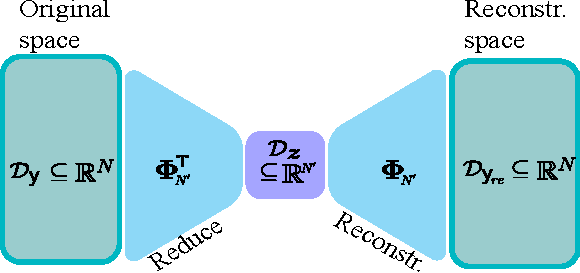
\includegraphics[width=90mm]{main_images/figure-PCA.pdf}
 \caption{ROM}
 \label{fig: ROM}
\end{figure}

Two commonly used approaches for high-dimensional spatial data are ROM and CNN. ROM techniques, such as proper orthogonal decomposition, reduce dimensionality by projecting outputs onto dominant eigenspaces identified via singular value decomposition, as illustrated in \Cref{fig: ROM}. The output is thus compressed into a latent space, with the number of retained modes determined by reconstruction accuracy. Spatial correlations are implicitly captured by the corresponding eigenvectors $\Phi$. Similarly, CNN learn nonlinear spatial representations through hierarchical filters, as shown in \Cref{fig: CNN}. Compared with ROM, the latent space in CNN is not necessarily of reduced dimensionality. Spatial structures are captured through convolution kernels and learned weights, and reconstruction is achieved via upsampling operations. While ROM and CNN handle spatial data using different algorithms, both operate within latent space. However, ROM requires an explicit DR technique, such as PCA, which could become challenging when output data is in tensor form, irregular, or of unequal length. Therefore, this study adopts a CNN-based method to capture complex nonlinear spatial patterns due to its greater flexibility. At the same time, a ROM approach is implemented as a baseline for comparison.
\begin{figure}
\centering
 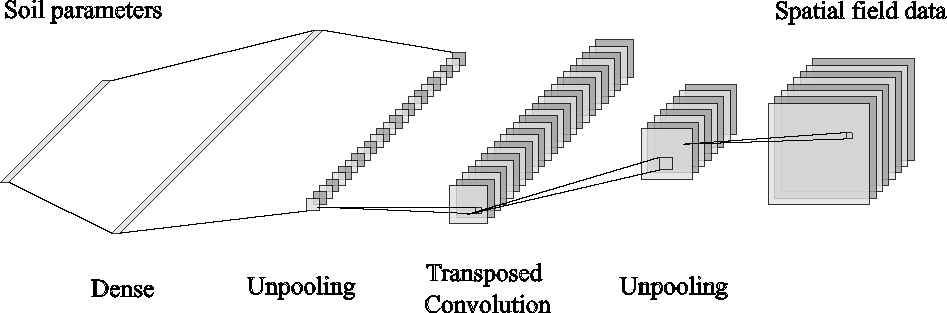
\includegraphics[width=90mm]{main_images/figure-CNN.pdf}
 \caption{CNN architecture}
 \label{fig: CNN}
\end{figure}




\subsection{Modelling temporal correlations via memory mechanisms}\noindent
LSTM networks are a specialised type of recurrent neural network designed to mitigate the vanishing gradient problem and to capture long-term dependencies in sequential data. As illustrated in \Cref{fig: LSTM}, the architecture comprises a memory cell regulated by three gates, input, forget, and output, that govern the flow of information. This design enables LSTM to retain and utilise relevant features across extended time horizons, making them particularly effective in sequence modelling tasks such as time series forecasting, stress history representation, and long-term monitoring \parencite{yu2015,benabou2021,qiu2025}.

In typical geotechnical modelling, input parameters such as soil properties are static, while outputs evolve over time. This discrepancy limits the applicability of standard LSTM networks, which require sequential inputs. To overcome this, a decoder-only architecture is developed to generate temporal responses conditioned on static inputs. This enables efficient emulation of time-dependent behaviour without relying on input sequences. Further details follow.
\begin{figure}
\centering
 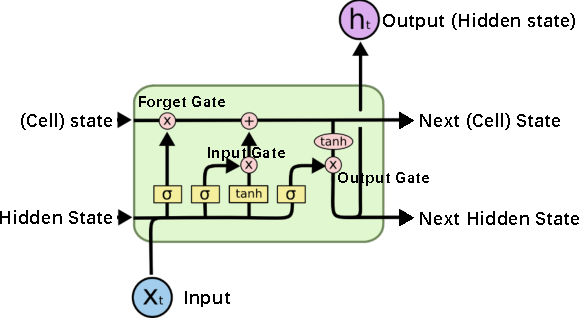
\includegraphics[width=90mm]{main_images/figure-LSTM.pdf}
 \caption{LSTM architecture}
 \label{fig: LSTM}
\end{figure}





\subsection{Simplified strategy to multi-field, multi-stage outputs}\noindent
As illustrated in \Cref{fig: decoder_only}, the static inputs are first transformed via fully connected layers to enrich and align features, then replicated across time steps before being passed to LSTM layers that capture temporal dependencies and produce latent sequences. These latent representations form an information bottleneck that bridges temporal decoding and spatial reconstruction. Spatial decoding is performed by specialised 1D or 2D convolution neural networks according to the output field type, with a TimeDistributed wrapper ensuring consistent decoding across time. When there is scalar output showing no spatial feature, only time-dependent layer is used. This modular separation of temporal and spatial components allows efficient and interpretable learning of evolving field patterns. Unlike typical sequence-to-sequence or encoder-decoder architectures (e.g., image sequences or climate fields), which encode time-varying inputs, the simplified design avoids unnecessary complexity by directly conditioning sequence generation on static inputs. Joint training of multiple output fields through a unified loss promotes balanced and coherent predictions. 

\begin{figure}
\centering
 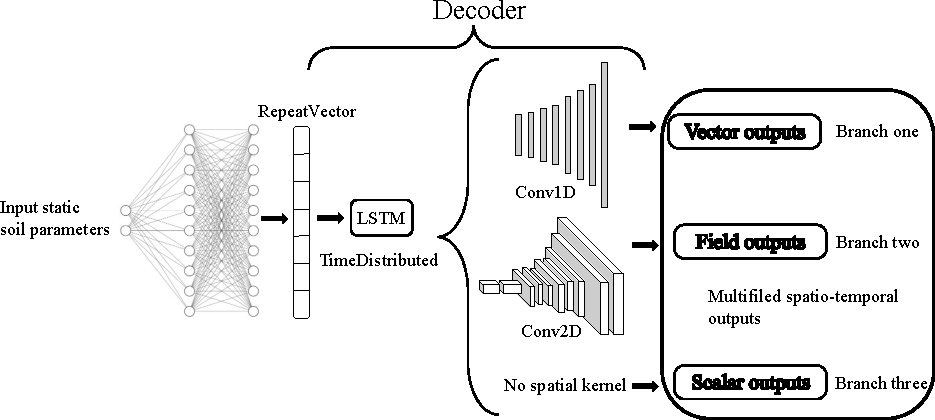
\includegraphics[width=140mm]{main_images/figure_NN.pdf}
 \caption{Decoder-only NN architecture}
 \label{fig: decoder_only}
\end{figure}


It is noted here different with ROM-surrogate frameworks \parencite{yang2024}, the proposed method avoids the two-step procedure of dimensionality reduction followed by surrogate modelling. This arises from the need to handle field outputs with non-uniform sequence lengths, as conventional reduction methods (e.g., principal component analysis, singular value decomposition) necessitate flattening the outputs into one-dimensional vectors, thereby disrupting their internal structure \parencite{sirovich1987,holmes2012}. Even advanced tensor-reduction techniques face compatibility issues with existing surrogate models, as the reduced formats are dimensionally inconsistent and ultimately still require flattening \parencite{kolda2009}. The proposed approach aims to offer greater practicality and ease of implementation for engineers.


In standard encoder-decoder formulations, the encoder is used to compress (or project) high-dimensional inputs and extract latent features, while the decoder reconstructs the high-dimensional outputs from latent representations. Such designs are well suited to problems with complex or structured inputs. However, many geotechnical engineering applications involve low-dimensional static inputs, such as soil parameters, for which an explicit encoding stage for input compression may be not essential. The proposed model therefore adopts a simplified (encoder-free) formulation in which static inputs are directly mapped into a latent representation, temporal dependencies are captured, and spatio-temporal responses are generated through the decoding components. It reflects that the primary modelling effort lies in decoding the latent representation into complex spatio-temporal outputs, rather than in performing deep feature extraction on the inputs.

\subsection{Testing the surrogate through a sequential inversion process}\label{sec: SBI}\noindent
The use of probabilistic back-analysis based on observations in geotechnical projects has been widely reported \parencite{hsein2013, lo2019, jin2021}. Among the different inverse approaches, such as maximum likelihood, maximum a posterior estimation and Monte Carlo simulation, Bayesian updating is regarded as particularly attractive for reducing uncertainties in soil parameters. Bayesian inference provides a rigorous probabilistic framework in which prior knowledge is combined with a limited number of observations. In this setting, soil parameters are treated as random vectors, with realisations denoted by $x$. The corresponding output responses are collected in a vector $y \in \mathbb{R}^{N}$, where $N$ is the length of the output. By applying the \textit{sum rule} and \textit{product rule} of probabilistic theory, the posterior distribution of the parameters $x$ can be expressed as:
\begin{equation}
\pi(x|y) = \frac{{\mathcal{L}(x|y) \cdot \pi(x)}}{{\pi(y)}} \label{equation Bayes},
\end{equation}
This expression, commonly known as \textit{Bayes' theorem}, defines the posterior distribution $\pi(x|y)$ in terms of the prior $\pi(x)$, the likelihood $\mathcal{L}(x|y)\stackrel{\mathrm{def}}{=}\pi(y|x)$
and the normalising constant, or evidence $\pi(y)$.

\Cref{equation Bayes} is rarely used, as computing the evidence $\pi(y)$ is typically intractable due to model complexity or high computational cost. Thus, methods which can approximate the posterior distribution are used. One common approach is to directly sample the posterior distribution using a Markov Chain Monte Carlo (MCMC) sampling algorithm \parencite{andrieu2003}. To avoid the computational burden of sampling using the forward model, MCMC simulations use a surrogate to construct a Markov chain ($x^{(1)}, x^{(2)}, \cdots )$ over the prior support $\mathcal{D}_{\boldsymbol{x}}$. In this study, the \textit{affine-invariant ensemble sampler} algorithm was used to construct the Markov chains with a burn-in period of 70\%. To speed up the inversion process and also at the same time verify the performance of the constructed surrogate, the surrogate model $\tilde{\mathcal{M}}(x)$ is embedded in the likelihood function. Assume that the \textit{uncertainty noise} term $\varepsilon_{r}$ follows a zero mean multivariate Gaussian distribution, i.e., $\varepsilon_{r} \sim \mathcal{N}(0,\Sigma_{\varepsilon_{r}})$. Given $m$ sets of observations and following the construction of an appropriate surrogate $\tilde{\mathcal{M}}(x)$, the likelihood can be explicitly expressed as:
\begin{equation} 
 \label{eq: modified_Likelihood function}
\begin{aligned}
 \mathcal{L}(x|\mathcal{Y}) =& \prod_{i=1}^{m} N(y^{(i)}|\tilde{\mathcal{M}}(x),\Sigma_{\varepsilon_{r}}) \\
 =& \prod_{i=1}^{m}\frac{1}{\sqrt{(2 \pi)^{N}{\rm{det}} 
 (\Sigma_{\varepsilon_{r}})}}\exp\left(-\frac{1}{2}\left[y^{(i)} - \tilde{\mathcal{M}}(x)\right]^{\mathsf{T}} \Sigma_{\varepsilon_{r}}^{-1}\left[y^{(i)} - \tilde{\mathcal{M}}(x)\right]\right) ,
\end{aligned}
\end{equation} 
\noindent The noise covariance matrix, $\Sigma_{\varepsilon_{r}}$, is mostly unknown and may be treated as additional unknowns that can be inferred jointly with the forward soil parameters. To characterise the noise, a diagonal covariance matrix of the form $\Sigma_{\varepsilon_{r}} = \sigma^2 \times \mathbf{I}$ with an unknown residual variance $\sigma^2$ is adopted, where $\mathbb{I}$ denotes an identity matrix. Although more complex noise representations exist and can be considered, this study adopts the simplest form for clarity and demonstration purposes \cite{hsein2013,lo2019}. For further details on sequential Bayesian calibration and uncertainty quantification, refer to \cite{yang2026}. 


In practice, geotechnical construction is typically carried out in stages, and it is therefore natural to employ a recursive updating strategy that reflects the sequential nature of the works. Within this framework, a sequential Bayesian calibration scheme can be applied, whereby soil parameters are progressively updated as additional observational data become available. This process allows the evolving parameter estimates to be incorporated into subsequent analyses, leading to predictions of key outputs, such as wall deflections or ground movements, with progressively reduced uncertainty at each stage of loading or excavation, as illustrated in \Cref{fig: SBI}. The updating can be repeated throughout the construction process, thereby providing a consistent mechanism to refine soil parameters and improve predictive confidence until project completion. It should be noted, however, that the initial generation of the training database relies on these FE simulations, and this upfront computational effort cannot be avoided; the surrogate and subsequent UQ analyses are inherently based on the results of high-fidelity FEM.

\begin{figure}
\centering
 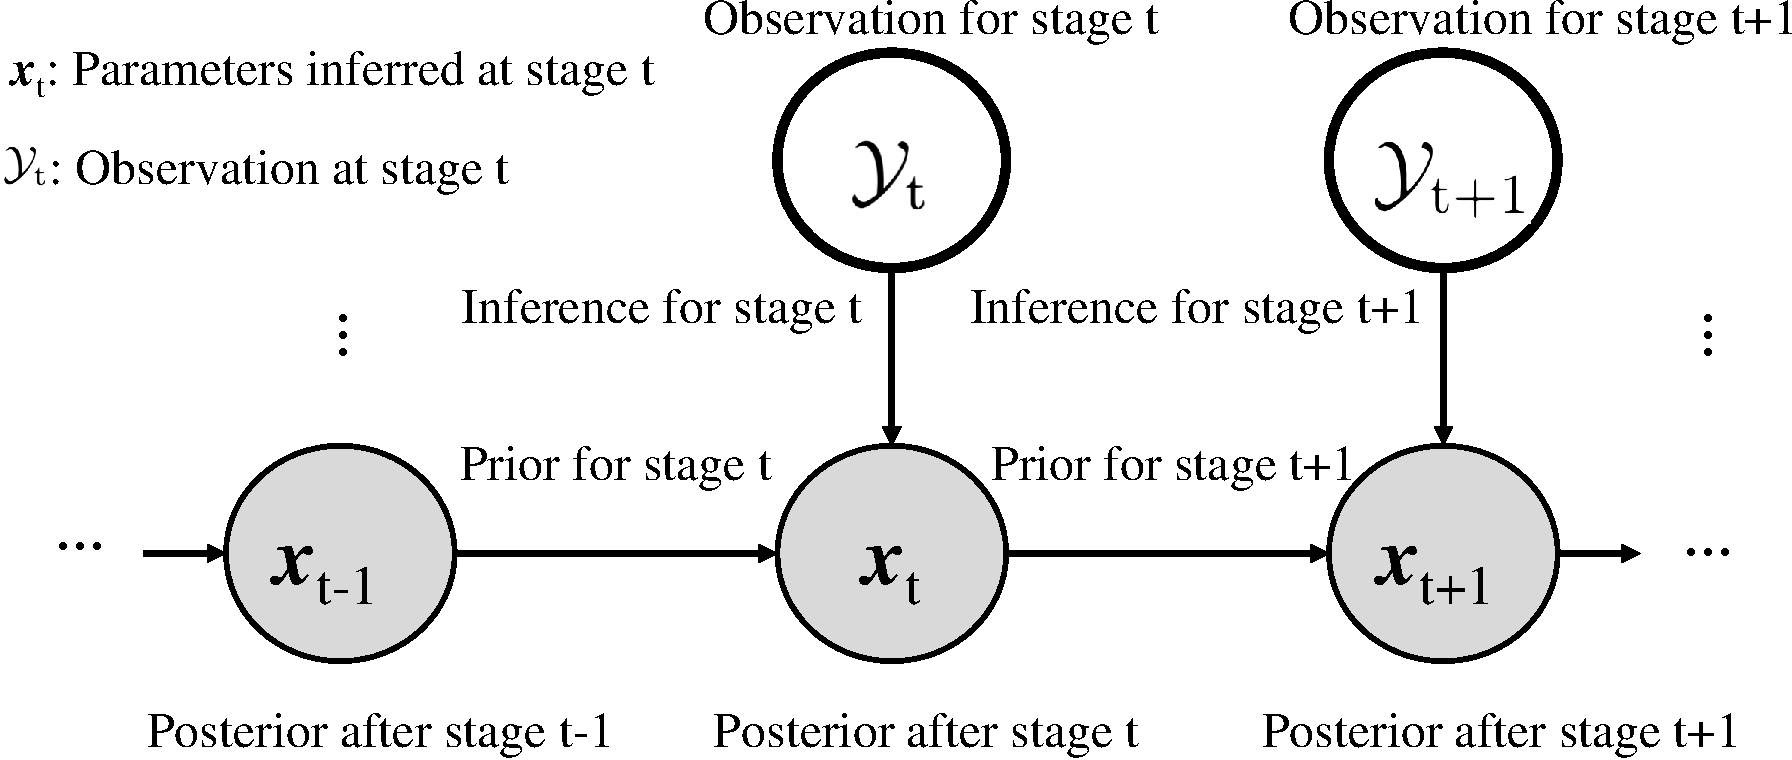
\includegraphics[width=90mm]{main_images/figure-SBI.pdf}
 \caption{Sequential Bayesian inference}
 \label{fig: SBI}
\end{figure}



















